\documentclass[11pt,a4paper]{article}
\usepackage{acl2015}
\usepackage{times}
\usepackage{url}
\usepackage{latexsym}
\usepackage{algorithm} 
\usepackage{algorithmic}
\usepackage{bm}
\usepackage{graphicx}
\usepackage{enumitem}
\usepackage{multirow}
\usepackage{todonotes}
\usepackage{tikz}
\usetikzlibrary{arrows}
\usepackage{caption}
\usepackage{subcaption}
%\newcommand{\rulesep}{\unskip\ \vrule\ }

\title{Semantic understanding of natural language text using distant supervision}
\author{Sudha Rao (raosudha@cs.umd.edu)}
\date{}

\begin{document}

\maketitle

\section{Motivation}

The beauty of natural language lies in the fact that it allows us to express the same thought in very different ways. But this makes it hard for machines to deal with natural languages since machines are good at memorizing data but pretty bad at generalizing from them. For e.g. a human can easily identify that the two sentences ``The boy wants the girl to believe him'' and ``The boy has a desire to be believed by the girl'' mean the same but it is difficult for a machine to do so. What can help machines in this case is if they can work with a kind of representation that abstracts away from various syntactic idiosyncrasies and captures the very meaning of the sentence. Such semantic level of understanding of text is becoming more and more necessary as the field of natural language processing (NLP) tries to solve problems that are closer to natural language understanding. Machines learn from examples and hence need annotated data to train on. However, annotating data with semantic information is expensive and time-consuming since it requires a linguistic expert in the loop. The availability of rich knowledge bases in recent times has given rise to an indirect way of gathering training data called distant supervision \cite{mintz2009distant}. In this technique, instead of annotating a sentence with information, given an information stored in the database, we gather sentences that may contain evidence for that information. 

My research work focuses on how we can use distant supervision technique for solving problems that require deeper semantic understanding of text. In subsequent sections I will discuss some of my work that fall under this category and also discuss how these ideas are relevant to some of the work at Adobe Research.

\section{Zero pronoun resolution}
I first came to appreciate the usefulness of distant supervision in my work on zero pronoun resolution for Chinese \cite{rao-EtAl:2015:NAACL-HLT},. Chinese being a``pro-drop'' language tends to drop pronouns when they are implicit from the context. This phenomena is more apparent in a dialogue setting since the speakers tend to refer to each other a lot. The corresponding task of resolving the dropped pronouns to one of the speakers (or to an outside entity in case of third person pronoun) is called zero pronoun resolution. In our work we developed a novel sequential model that explicitly tracked the conversation focus in a dialogue and used that to resolve the zero pronouns. To train our model, we needed annotated data and it was expensive to have humans annotate data for us. English unlike Chinese is not a pro-drop language and mentions pronouns explicitly. Also there is huge amount of readily available Chinese-English parallel corpora. So in our work we developed a method to automatically annotate the training data using the pronouns in the English translation of the Chinese sentence, allowing us to have a large amount of data to train on. This kind of a distant supervision, even though noisy, turned out to be very useful for our task and gave significant improvements over purely supervised approaches.

\section{Relation extraction}
Given a text, identifying who did what to whom has been an important task in NLP. This problem becomes even more challenging when the text expresses multiple hierarchical relations in a complex manner. For e.g. consider the following sentence from biomedical literature - `` This LPA-induced rapid phosphorylation of radixin/moesin was significantly suppressed in the presence of C3 toxin, a potent inhibitor of Rho''. As humans we can identify the various complex relationships in this text but for a machine to do so, it needs a deeper semantic representation of the text. Abstract Meaning Representation (AMR) \cite{banarescu2013abstract} in one such semantic representation that tries to capture the overall meaning of the sentence in the form of a graph structure. Figure ~\ref{amr_eg} shows the AMR corresponding to the previously mentioned sentence. Identifying the right relations is much easier for a machine now given the AMR structure as opposed to when it was given just the original sentence. During summer 2015, I worked with Dr. Daniel Marcu and Dr. Kevin Knight at ISI on developing methods for relation extraction from biomedical text using AMR. Existing supervised methods for relation extraction gave a low recall on this task. We hypothesized that the key reason for this was the low amount of training data. Biomedical domain has a rich source of knowledge bases that contain information about protein-protein interactions. Additionally, it also has millions of research papers published over the years that talk about such protein interactions. We made use of these resources to gather a large amount of additional training data using the distant supervision technique. It has been shown that training data gathered using distant supervision can be noisy sometimes \cite{takamatsu2012reducing}. Hence, we made use some path heuristic in the AMR of the sentence to label them more cleverly. This work lead to a system with high recall of 0.75 (F1 0.49) over a baseline recall of 0.23 (F1 0.32). Currently I am working on building deep neural network that can further exploit the AMR graph structure.

\section{Future work}
Syntactic representations like constituent parse trees and dependency parse trees have been successfully used for solving many problems in NLP for a long time now. But equivalent semantic representations like AMR have been less explored. One of the main reasons for this is the lack of automatic parsers that can accurately parse sentences into such semantic representations. Recently there has been a lot of work on AMR parsing \cite{flanigan-EtAl:2014:P14-1}, \cite{pust2015using}, etc. But the accuracy of these parsers is much lower than those we get for syntactic parsers (e.g. dependency parsers). One of the main reasons for this is the paucity of annotated data. Semantic annotation requires much deeper linguistic expertise than any kind of syntactic annotation and hence is time consuming and expensive. One might go as far as saying that huge amounts of semantically annotated data might never be available for machine learning models to efficiently learn from. But humans do not need such huge amounts of data to efficiently parse a sentence for its sentence. They can generalize much better. How do they do that? There has been a lot of work in linguistics to show that humans make use of context and common sense knowledge while parsing a sentence for its meaning. Can machines do something similar? Wikipedia, DBPedia, OpenCyc, Freebase, etc. are some examples of knowledge bases that machines can make use of. We have already seen the potential of distant supervision to solve semantically challenging tasks and so in future I plan to explore how we can leverage the information stored in such knowledge bases to improve semantic parsing using distant supervision techniques.

\begin{figure}
\centering
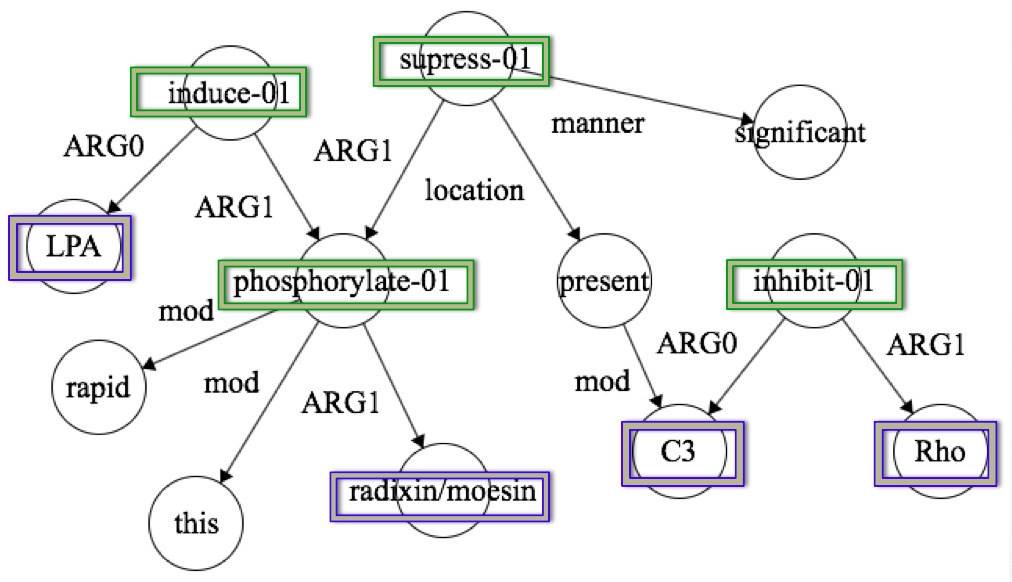
\includegraphics[width = .5\textwidth]{EgAMR}
\caption{AMR for sentence ``This LPA-induced rapid phosphorylation of radixin/moesin was significantly suppressed in the presence of C3 toxin, a potent inhibitor of Rho''}
\label{amr_eg}
\end{figure}

\section{Applications to Adobe }
I believe that my current expertise in semantics puts me in a good position to contribute to the ongoing research in text analytics at Adobe. In recent times the combination of vision and natural language processing has been successfully used for solving many interesting problems. One specific project at Adobe that caught my interest was: Editing images with natural language \cite{laput2013pixeltone}. Interpreting user commands can be challenging when they go from simple ones like ``make it bright'' to more challenging ones like ``the image needs to be bright'' or ``the image is too bright'' which need better semantic interpretations to understand that the action required in the two cases are completely different. Making use of semantic representation to parse the phrases can ease the task of interpretation and help provide a platform where users can express themselves more naturally. Contextualized advertising system based on text is another area that can benefit from deeper semantics. Recommending truly relevant ads to the user requires an understanding of the text that is deeper than just a keyword match.  

\bibliographystyle{acl}
\bibliography{ResearchOverview}

\end{document}


